\documentclass{article}
\author{
  Torrent Gorjon, Xavier\\
  \texttt{Xavier.TorrentGorjon@os3.nl}
}
\title{Protecting against relay attacks forging increased distance reports}

\usepackage{graphicx}
\usepackage[backend=bibtex]{biblatex}




\bibliography{references}


\begin{document}


\begin{titlepage}
\center
\textsc{}\\[1cm]
\textsc{\LARGE Universiteit van Amsterdam}\\[1.5cm]

\textsc{\Large Research Project I}\\[0.5cm]

\textsc{\Huge Protecting against relay\\[0cm] attacks forging increased\\[0.5cm] distance reports}\\[1.5cm]


\includegraphics[scale=1]{images/uva.png}\\[1cm]

\begin{minipage}{0.5 \textwidth}
\begin{center} \large
Xavier Torrent Gorj\'{o}n\\
\emph{Xavier.TorrentGorjon@os3.nl}\\[0.5cm]
\end{center}
\end{minipage}\\[2cm]
{\large \today} 


\end{titlepage}


\newpage


\renewcommand{\abstractname}{\Large Abstract}
\begin{abstract}
Distance-bounding protocols have been for a long time a research topic due their usefulness as a security feature for systems that assume a specific proximity between parties. However, no studies could be found in the current literature regarding attacks that fake increased distance reports.

This research project first discusses alternative solutions using other systems such as radar and GPS. An analysis on why these systems are not enough to solve the problem in the current state of the art is provided.

Afterwards, some real world scenarios are presented, in which the security of these applications could be compromised. An explanation of how relay attacks could interfere the expected behaviour of these systems is provided, followed by an evaluation of the consequences it might have for each one of them.

Some low-cost, easy-to-implement solutions are proposed, which greatly diminish the success chances of this kind of attacks against this protocol.
\end{abstract}

{\bf Keywords --- Relay attack, distance-bounding protocol} 

\newpage

\section*{Glossary}
\addtocounter{section}{0}

\begin{description}
  \item[GPS] Global Positioning System: Navigation system based on satellite communication maintained by the United States government.
  \item[INS] Inertial Navigation System: Navigation system that keeps track of the route used by an object to have awareness of its location.
  \item[LIDAR] Light Detectiong and Ranging: Object-detection system based on laser.
  \item[MANET] Mobile Ad-Hoc Network: A network of independent devices deployed for a specific purpose.
  \item[RADAR] Radio Detecting and Ranging: Object-detection system based on radio waves.
  \item[RCS] Radar Cross Section: Signature of an object on a radar system.
  \item[ToF] Time-of-Flight: Measurement on the time required to receive a signal response from another party after a signal is sent.
\end{description}

\newpage



\tableofcontents





\newpage








\section{Introduction}
\label{sec:introduction}

Communications between machines face many challenges when the transmitted information needs to be protected. Most communications can prove to be valuable attack points for third parties that want to recover, modify, block or otherwise manipulate the original message sent for personal profit. Part of these attacks can be prevented by using end to end encryption and signature of the data. However relay attacks cannot be prevented just by using cryptographic algorithms.

Relay attacks consist on the mere reception and replay of information. Although at first this might seem harmless, many systems become vulnerable if that relaying of information is not noticed. One scenario that can be used as an example of the threat these attacks represent are access control systems, in which a device is used to prove that a user is within a certain distance from a validator through a challenge-response protocol. On unprotected implementations of these access control systems, an attacker can relay the challenge from the validator to a valid user who is not in range and relay its answer back to the validator, effectively bypassing distance validation. Practical attacks on this kind of systems have been demonstrated on various studies, as in \cite{francillon2011relay, francis2010practical, hancke2005practical, markantonakis2012practical}.

In this paper, we will first discuss the relay attacks used to forge fake location positions, focusing on the countermeasures against them. We will then focus on attacks forging increased distance reports, the feasibility of these attacks and propose solutions to them. In Section \ref{sec:relatedwork} we discuss the available literature on this topic. In Section \ref{sec:background} we briefly present results and conclusions from our research in the available literature about distance bounding protocols, GPS, radar detection and Inertial Navigation System. We present in Section \ref{sec:researchquestions} a more detailed explanation on the research questions this project aims to answer. Following in Section \ref{sec:methodology} we explain the methodology used in this study. Section \ref{sec:results} discusses the actual results from our research questions, after which we will provide conclusions about the results gathered in Section \ref{sec:conclusions}.







\section{Related Work}
\label{sec:relatedwork}

Relay attacks have been for long, and continue to be, an extensive field of research, as technologies and devices are shifting to a more mobile-focused paradigm. Many old procedures are being enhanced with wireless features, such as credit cards and car keys. However, we could not find in the available literature studies regarding relay attacks used to fake increased distances between two legitimate nodes. It is the goal of this project to prove that these attacks can prove to be a huge threat to real world applications using these systems, and how current distance bounding protocols can be enhanced to limit their vulnerability against them.

There is much literature available presenting solutions to distance bounding problems \cite{brands1994distance, tu2007rfid, rasmussen2010realization}. All of these studies are used as a basis for others in a constant iteration to improve the protocols. As new attacks emerge against distance bounding protocols, new studies are published to fix the deficiencies of the previous work. This project will use part of these studies as a basis for the solutions against the studied relay attacks.

There are also many practical studies in the field of distance bounding, which aim to test the vulnerabilities on real applications\cite{francillon2011relay, francis2010practical, hancke2005practical, markantonakis2012practical, vandenbreekel2014relay}. Although all these refer to forging decreased distance reports and it is not directly used in our research, it has been deeply useful as a starting point and inspiration.

This project will assume certain conditions for the studied attacks. Some assumptions and justifications will be required on the investigation, based on the characteristics of GPS signals. Many studies focus on the feasibility of intentional attacks against GPS systems\cite{warner2003gps, wen2005countermeasures, jafarnia2012gps}. These studies conclude that, even though spoofing is hard with the solutions they propose, it is not impossible. With this premise, the goal will be to develop countermeasures against relay attacks without relying on GPS signals.

In a similar way to GPS signals, other systems such as Radar location \cite{cadirci2009rf} and Inertial Navigation Systems \cite{patent:4085440} could be arguably used to prevent this attacks. Using these information sources we will explain why these systems are not reliable neither, reaffirming the need of a modified distance bounding protocol that is not vulnerable to relay attacks.

Finally, this study is closely related to the field of MANETs (Mobile Ad-hoc NETworks), and as such, literature available in this topic is of our interest. In particular, wormhole attacks (\cite{hu2006wormhole, maheshwari2007detecting, goyal2010literature}) are a specific type of relay attack that, while being different than the ones we will study in this document, provide insight to our investigation as they are closely related.








\section{Background}
\label{sec:background}

In this section we will discuss distance bounding protocols, the GPS system and radar detection. All of them are relevant topics to our research. First we will explain the current distance bounding protocols, as we will use them as a starting point for our research. Then we will move on to GPS, and explain why systems shouldn't rely completely on it, hence the need to develop more powerful distance bounding protocols for our study cases. Lastly, we will discuss the possibility of using radar detection and Inertial Navigation System to fight the proposed attack.

\subsection{Distance bounding}

Distance bounding protocols were developed as a response to relay attacks that attempt to fool systems that validate an users proximity to a validation point. Common scenarios of these applications are found in access control systems, such as smartcards to access buildings or cars using remote passive keys.

These attacks try to use properties of the systems used in the communications (such as signal intensity or message time of flight (ToF)) to validate the proximity of users. Based on the previous studies available\cite{capkun2006secure}, we will proceed to briefly discuss these methods:

\begin{description}
  \item[Signal Intensity] Signal intensity protocols try to achieve proper location of other nodes by measuring the received signal strength. Previous work available in the public literature\cite{seshadri2005bayesian} proves the usefulness of this location system. Even though attacks on this systems are hard to perform \cite{sheng2008detecting}, the defences against them rely mostly on anomaly detection. The reliability of these systems can be decreased in heavily adverse situations, and the ToF methods discussed next provide a higher degree of security.
  \item[Ultrasound ToF] Ultrasound ToF measures the round-trip time of messages sent and received from the parties measuring the distance between them. This does not depend on the signal strength for the measurement, although ultrasound-based ToF has the latent vulnerability that other methods such as radio frequency or optical wires attackers can surpass the speed of the ultrasound communication, effectively being able to relay information faster than the legitimate infrastructure\cite{capkun2006secure}.
  \item[Radio ToF] Radio-based ToF uses the same method as ultrasound ToF to perform the distance check. The key of the success of this method is that the information transmitted travels at speeds near the speed of light, meaning there is no physical way to fake one node is closer than it really is. Practical studies on this method \cite{rasmussen2010realization} developed hardware that can perform the operations required under 1ns, meaning that the maximum theoretical distance an attacker can shorten its reported distance is under 15cm.
\end{description}

In this project we will be using Radio ToF as a basis for our work, as it is proven to be the most secure and reliable method. However, this method alone is not enough to fight reports that forge an increase on the real distance between parties, and this will be the main focus of our research.

\subsection{GPS location}

It could be argued that GPS location can be used to prevent the attacks that we will discuss on the next Section. However, GPS signals have their own weaknesses both with and without presence of adversaries.

In settings without adversaries, GPS positioning cannot be reliably used indoors or underground, and sometimes the presence of tall buildings or structures nearby is enough to disrupt its data.

Speaking of scenarios with one or multiple adversaries, even though there are many countermeasures to prevent attacks against GPS positioning \cite{warner2003gps, wen2005countermeasures, jafarnia2012gps}, there do not provide complete security, similar to the Signal Intensity location protocol.

Due these problems, he U.S. government actually recommends to always have backup systems for GPS and suggests to never rely entirely on it\footnote{\url{http://www.gps.gov/support/faq/#jamming}}. Based on these premises we will assume that GPS is not a part of our system, or that we cannot rely on it.

\subsection{Radar detection}

One way to protect against this kind of Man-In-The-Middle attack could be by attempting to physically detect the attacker. If an unidentified object is detected between the parties and it is confirmed that it does not belong to the system, security measures could be taken to prevent such relay attacks.

However, recent studies as the one by \citeauthor{cadirci2009rf} in \cite{cadirci2009rf}, state that Radar Cross Section\footnote{\url{http://www.microwaves101.com/encyclopedia/Navy handbook/4.11 Radar Cross-Section (RCS).pdf}}, a measurement used to rate the ability to reflect radar waves by an object, can be heavily decreased by employing proper techniques such as the usage of special materials, radiowave-absorbing paint and specific shapes that minimize and disperse radio reflection.

As a real world example, the first operational aircraft designed to employ advanced stealth technology, the Lockheed F-117 Nighthawk from the United States Air Force, with a wingspan and a length of $13.20m$ and $20m$ respectively\footnote{\url{http://www.fighter-planes.com/info/f117_nighthawk.htm}}, has a RCS signature of $0.025m^2$, which is similar to that of a bird\cite{cadirci2009rf}.

In the attack scenarios proposed in Section \ref{sec:results}, flying drones would be the most versatile device to perform the attacks. Considering these drones can be considerably smaller than these aircraft (depending on the situation, the used drone could be shorter than $1m$ in length, height and width), it is easy to foresee that they would be almost invisible to radar systems. If the attack scenario does not require the attacker to fly at relative high speeds, its RCS signature could be further decreased by designing an attack drone with a shape specifically made to absorb radar waves. 

We therefore conclude that, in the current state of stealth and anti-stealth technologies, radar detection would not be a strong countermeasure to prevent against that kind of attacks.



\subsection{Inertial Navigation System}

Inertial Navigation Systems are devices used to provide machines a sense of self-awareness of their current position, based on their initial position and the chosen routes, by using accelerometers and gyroscopes. These systems could be relevant for this research, as they share the same \emph{relative positioning} focus, staying independent from third party sensors.

The work done by \citeauthor{woodman2007introduction} in \cite{woodman2007introduction} evaluates the cost and performance of the INS. The conclusion from that work is that available INS hardware cannot realistically provide an accuracy below $5m$ of error after $60$ seconds of operation. In an environment with multiple nodes using this system, this means that after $60$ seconds, the location detection between two nodes could be as biased as $10m$. This also limits is usability as a stand-alone positioning system, as the error will only grow larger as time goes on.

Although INS accuracy is rapidly improving over the years, right now is not a viable solution or countermeasure to our problem.







\section{Research Questions}
\label{sec:researchquestions}

As seen in the Related Work section, in the current literature there are no proposals to fight the subset of relay attacks that attempt to fake increased distance reports between legitimate parties. This project will first study the difficulty of performing these attacks. Therefore, our first research question will be:\\

\emph{How feasible are forged increased distance report relay attacks?}\\

Minimum distance bounding appeared to have many solutions on the current literature. However, we observed that distance bounding regarding upper limits on reported distances was not a subject of research. In this project, we will present some theoretical attacks that could be used on many real world scenarios, and propose variations on the current distance bounding protocols to solve them.

The proposed scenarios are diverse in both context and properties of the systems involved in the communications. We will focus the study from the point of view of systems involving communication between drones, although we will provide solutions that can be extrapolated to other systems as well, such as automatically driven cars.

In this research question, we ultimately aim to explain how these attacks are relevant and under which circumstances they could be executed. If the results from this research determine that these attacks can pose a threat, we will consider a second research question:\\

\emph{How can forged increased distance report relay attacks be prevented?}\\

This second research question will focus on providing solutions to the issues stated on the first. Unlike minimum distance bounding protocols, we won't be able to use the speed of light as a fact to develop responses that cannot be faked, which implies that we might not be able to develop a system that completely protects against these increased distance reports. However, we do expect to provide solutions that could suppose a meaningful security increase against these attacks.









\section{Methodology}
\label{sec:methodology}

As stated in Sections \ref{sec:introduction} and \ref{sec:relatedwork}, there are reasons to see relay attacks that fake increased distance reports as a threat.

Using the information gathered and stated in the Background section, we will first study the conditions under which distance bounding systems could be vulnerable to these attacks. We will present various real life applications of distance bounding protocols whose intended functionality could be altered by performing these attacks.

Afterwards, using the mentioned sources of information, variations to the distance bounding protocols will be proposed, in order to effectively reduce the threat these attacks pose.

Using a theoretical approach, an explanation and evaluation of both the feasibility of these attacks as well as the proposed solutions will be given.











\section{Results}
\label{sec:results}

\subsection{How feasible are forged increased distance report relay attacks?}

The theoretical attack we propose relies on the fact that the discussed protocols regarding distance bounding on the available literature do not prevent relay attacks that report an increased distance between two legitimate parties.

The basics of the attack are easy to understand. Assume two parties are communicating using a transmitter-receiver model, that is, one of them is actively reporting its position to the other, using the Radio ToF distance-bounding protocol\cite{rasmussen2010realization}. At some point, an attacker seizes a position between them and starts disrupting the communication between them, either by attempting to block the communication or by jamming its frequency range. At the same time, he starts recording the information and resending it to the receiver node, adding a brief delay on it. Figure \ref{fig:attackexample1} provides a graphical description of the problem. The effectiveness of this attack can be increased by having multiple malicious nodes attempting to block the original signal.

\begin{figure}[h!]
  \centering
    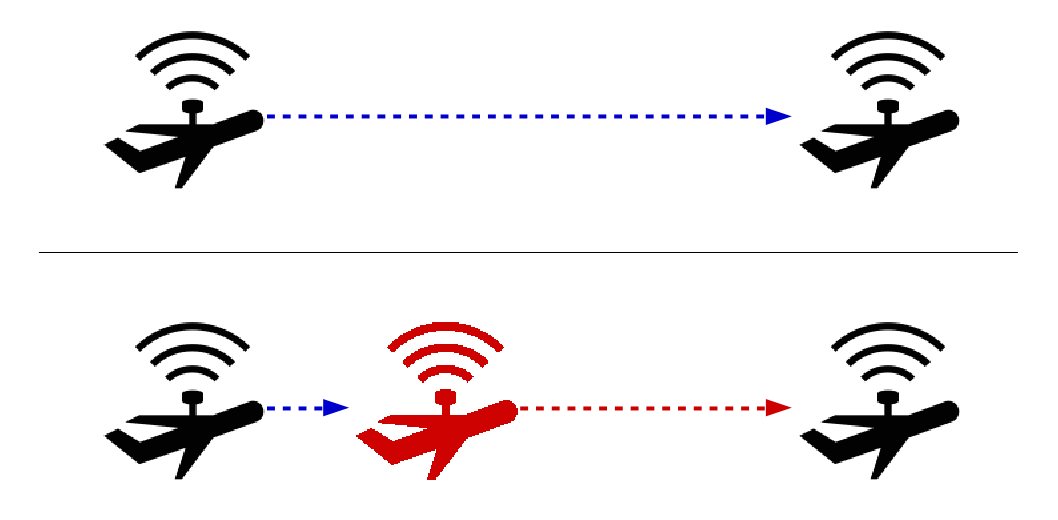
\includegraphics[width=0.8\textwidth]{images/attack1.png}
  \caption{Regular communication versus block and relay attack.}
  \label{fig:attackexample1}
\end{figure}

Many systems use these distance reporting protocols for their pathing decisions. This kind of attack could cause unexpected behaviour on the systems, effectively altering their original desired outcome. 

Such attacks are difficult to perform in practice, as they require relaying and jamming communications at the same time. Appropriate timing on the relay and some degree of knowledge about the system are also required to successfully perform an attack. However, there is no proving that these attacks cannot be performed with the appropriate technology.

Following next, we will discuss some real world applications that may be interesting for this research.

\subsubsection{First example of real world attack: Autonomous cars}

Autonomous driving is a topic that is receiving a lot of attention by many researchers around the globe in recent years. The variety and quantity of studies on this field \cite{franke1999autonomous,continentalautonomous,levinsontowards,geiger2012we}, prove its relevance as an interesting subject from the point of view of computer vision and location systems.

These autonomous cars use multiple systems to check and validate their position and the layout of the surrounding area. Usually these systems include a subset of GPS location, lasers, radars and computer vision systems\cite{continentalautonomous,levinsontowards}.

Distance bounding protocols seem to not be an active part of these systems, although they could be useful. First of all, the most obvious utility would be to provide an additional security layer to the system, providing additional means to locate other vehicles in normal conditions, or as a backup system in case other devices fail. This feature could be used as well to detect pedestrians in a future if devices such as mobile phones were adapted for this purpose.

Autonomous driven vehicles could also use distance bounding protocols to perform distance verification of specific targets. The distance bounding protocols developed in  \cite{rasmussen2010realization, capkun2006secure} can be used to check the distance with specific targets. This is interesting in this environment as in a high traffic road it is difficult to keep track of other specific vehicles through the use of lidar\footnote{Lidar is a laser-based detecting system: \url{https://lta.cr.usgs.gov/LIDAR}} or computer vision system.

Although the introduction of these distance bounding protocols on autonomous cars could prove to be useful for these purposes, it would also add a vulnerability in the form of the previously mentioned reported distance increase relay attacks.


\subsubsection{Second example of real world attack: Drone MANETs}

In the recent years there has been a huge increase on the interest towards drones\footnote{\url{http://www.google.com/trends/explore#q=drone}}, due the emergence of topics such as Amazon Prime delivery drones or the usage of unmanned aircraft by the US military.


\begin{figure}[h!]
  \centering
    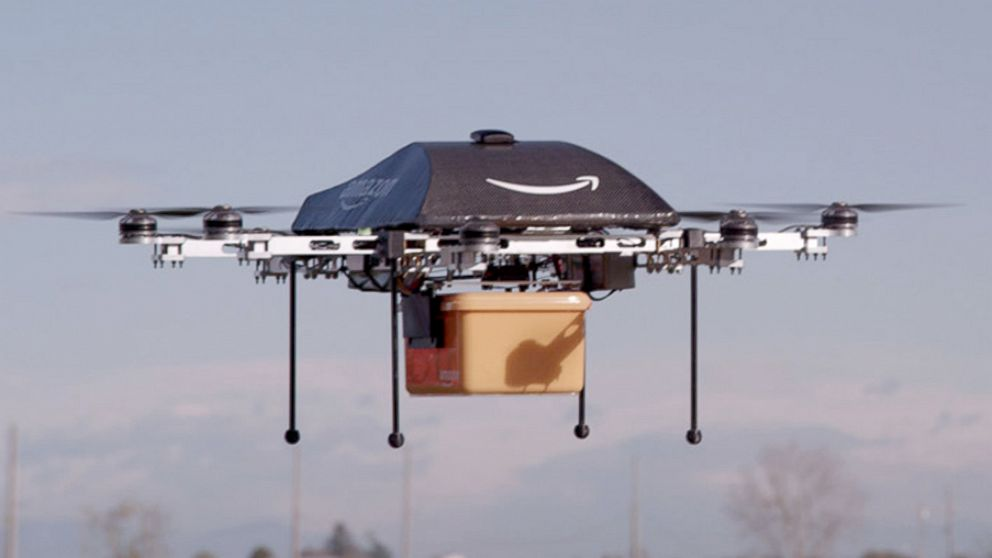
\includegraphics[width=0.6\textwidth]{images/amazonprimedrone.png}
  \caption{Amazon Prime delivery drone carrying a package. Because of legal constraints this delivery system is not being used yet, although it may start to be available at some point in 2015.\protect\footnotemark[5]}
  \label{fig:amazondrone}
\end{figure}

\addtocounter{footnote}{1}\footnotetext{\url{http://abcnews.go.com/Technology/amazon-prime-air-delivery-drones-arrive-early-2015/story?id=21064960}}

It is safe to foresee that that the usage of drones will only grow on the upcoming years due their ability to decrease costs and improve the performance of systems currently manned by humans. We present two scenarios on which the use of drones can be interesting and how can they be affected by the discussed relay attacks.

\begin{description}
  \item[Cooperative working drones] Taking as an example the Amazon Prime delivery drones, we can discuss the possibility of having multiple drones working in groups. One interesting scenario is the case of multiple drones carrying a huge package. For a company trying to keep expenses low, it would make sense to use multiple drones that can work cooperatively in different situations rather than having drones of various sizes for each type of package. In this situation, an attacker could try to attack that system by faking some drone's distance reports to the others, which may force the drones to change positions and loose equilibrium, eventually crashing.
 
  A relay attack on this platform could make more sense than just attempting to shut down the drones to achieve the same goal, as it would be extremely difficult to prove that a relay attack took place by checking the logs of the crashed drones. This could lead to a reputation loss for the delivery company, as their system would be seen as unreliable by the customers.
  
  
  \item[Area surveillance drones] Another common usage of drone MANETs is to perform area surveillance. This case has both civilian and military applications. Civilian uses range from searching missing people to area mapping, while military uses usually imply area reconnaissance searching for possible threats or targets. 
  
  In this particular situation where a group of drones is checking a zone, an attacker could attempt to interfere in the reported distances. This could cause the drones to believe they are further apart between themselves than what they really are. Under these circumstances, they could decide to get closer together so they do not leave zones unchecked between them, which would inevitably cause a reduction on the covered area. Figure \ref{fig:attackexample2} represents an example of this attack.
  
  \begin{figure}[h!]
  \centering
    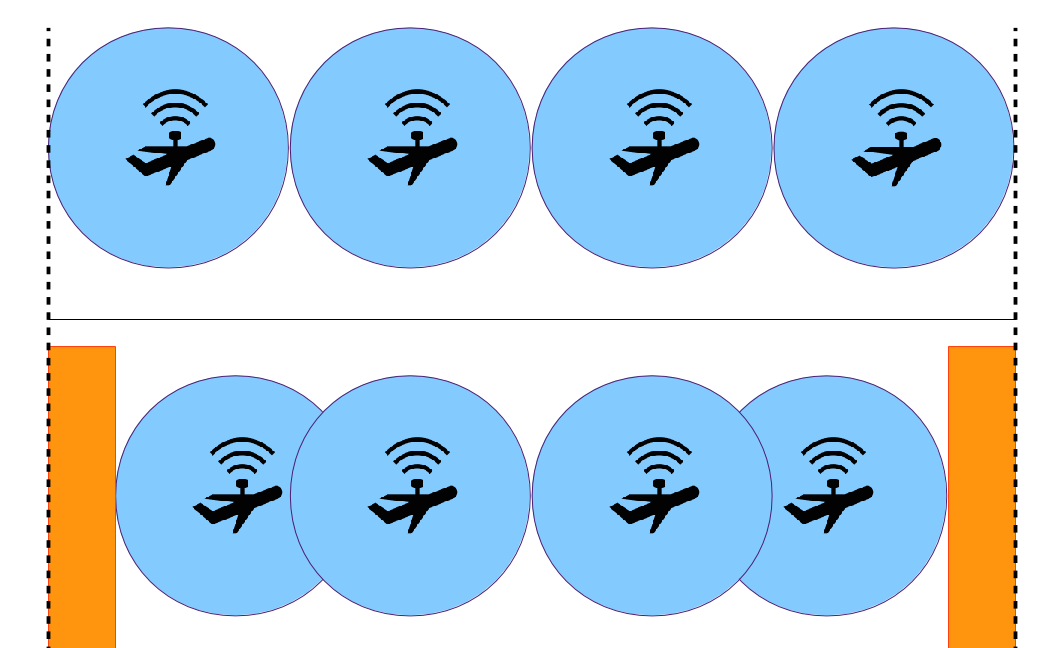
\includegraphics[width=0.8\textwidth]{images/attack2.png}
  \caption{Example of the proposed attack. On the first case, the four drones manage to explore all the expected area (marked with trailing dots). On the second, the marked zones on the sides represent the resulting unchecked area as a consequence of this attack.}
  \label{fig:attackexample2}
\end{figure}

This attack might prove considerably difficult to perform, but can have catastrophic consequences if successful. Unlike the attack on cooperative drones, distance is less of a restriction here, but in this case the attack requires a much deeper knowledge of the attacked system.

\end{description}


\subsection{How can forged increased distance report relay attacks be prevented?}

In this section some countermeasures to the studied relay attacks are proposed. These solutions can stack with one another and, in fact, it is recommended to do so, as each one of them provides an additional layer of security.

These solutions do not need new protocols or hardware, and instead rely on the replication and addition of redundancy to provide protection against the fake increased distance reports. This means that the systems discussed on the first research question could implement these with minimal modifications.

\subsubsection{Introducing behaviour verification}

Nowadays storage is hardly a limitation for systems, as the price, size and weight of these components has decreased to the point where multiple gigabytes of information can be stored in inexpensive memories that have the size of a screw.

Therefore, storing information on the recent location history of one or multiple parties is feasible. Uncoordinated attacks would be prevented with this feature, although it does little to protect against carefully planned ones. All location systems must allow some degree of variation on the measurements, as there may be many reasons for a slight delay in a communication. By successfully using that error margin, an attacker could still attempt to fake distance reports increasingly over a period of time.



\subsubsection{Utilize multiple distance-bounding signals}

Historically, distance-bounding protocols are used to validate an upper-bound distance between a prover and a validating station. As such, the exact location of a prover is not required, only its distance to the validating station matters (that is, check if the prover is within a certain circle of the prover in a 2D scenario, or a sphere in a 3D scenario).

If the nodes using distance-bounding protocols are large enough, multiple distance-bounding antennas can be used so that no only the distance from another node is known, but also its approximate location on the 3D space.

By using this triangulation system, attackers need to temper the communication between several antennas at the same time. Coupled with the behaviour verification solution, it becomes easier to detect relay attacks. For an attacker it is still easy to produce fake distance reporting positions on the same vector of the legitimate prover, but it becomes increasingly difficult to fake positions that diverge from that line. 

Figure \ref{fig:attackexample3} provides a graphical explanation of this defence mechanism. An attacker cannot make the left drone believe that the legitimate drone is inside the circle area, due the original distance-bounding protocol features. With this method an attacker can still fake a position in the darker area with relative ease, but faking a position outside from it becomes increasingly difficult as multiple distance reports have to be taken into account, and a deviation on any of them could end with the checking drone detecting inconsistency in the received data.

  \begin{figure}[h!]
  \centering
    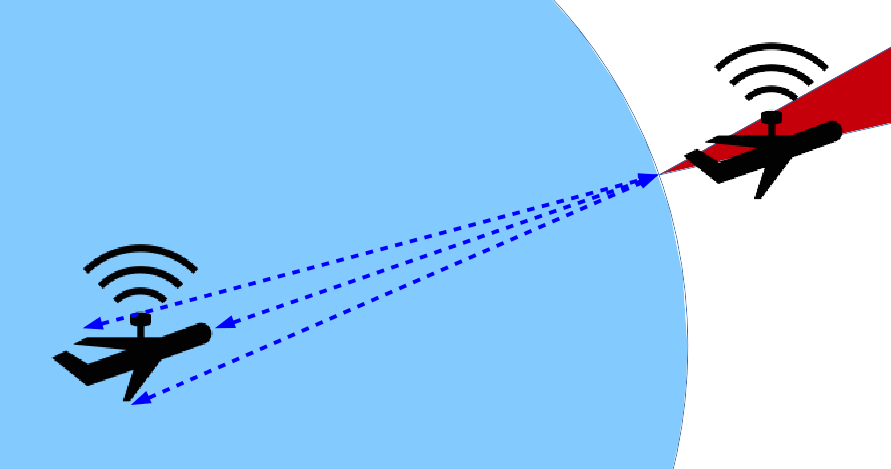
\includegraphics[width=0.8\textwidth]{images/attack3.png}
  \caption{Scenario after the proposed countermeasure.}
  \label{fig:attackexample3}
\end{figure}

This protection method has two major downsides. The first is that devices should carry more antennas, increasing their cost. Additionally, the device using this system needs to have a minimum size for it to be reliable, as the antennas need to be at a certain distance from one another to obtain a correct triangulation (otherwise the error margins would outweigh the correctness of the obtained distance values)

\subsubsection{Avoid centralized systems: distributed knowledge}

When the first attack definition was proposed on Figure \ref{fig:attackexample1}, only one of the nodes was reporting its location to the other. Although this setup may simplify the operation and decision-making of these nodes (by having only one node in the system taking decisions for the others), it also makes the system more vulnerable to relay attacks.

If all nodes on the system can share information of the position of neighbour nodes between themselves, an attack on the system becomes considerably more difficult to perform. In essence, this solution is similar to the previous one, but on a larger scope. It is not required that one node checks the distance between him and another one with all the other nodes on the system, although every additional node verifying the information makes it harder to perform an attack on the system.

This trade-off between communication load and security is the only restriction on this solution. Different applications will have different needs, and the delay between messages has to be considered as well (a node A can report to B the position of a third node C on a given time, but B must consider the delay of the transmission with A when checking the received data).










\section{Conclusions}
\label{sec:conclusions}

From the results on the first research question we can conclude that, even though the explored scenarios are only a subject of investigation right now and have no commercial use at the moment of writing this document, they will surely be amongst the most important developments in the upcoming years. This makes the vulnerabilities on distance-bounding protocols a latent problem.

As systems like the drone delivery and automated cars are not yet available to the open public, is it difficult to foresee what systems and protocols these platforms will use. However, in this document the usefulness of including distance-bounding protocols on them has been explained, focusing on the consequences distance-amplification attacks might have on them.

Multiple solutions to these distance-amplification attacks have been proposed and discussed. Even though upper-distance bound cannot be solved as lower-distance bound by using limitations on the information travelling speed, the proposed solutions noticeably decrease the chances of a malicious party successfully attacking the protocol.




















\section{Acknowledgements}
\label{sec:acknowledgements}

We would like to thank Jordi van den Breekel and Paul van Iterson, supervisors of this project at KPMG, for their support over the duration of this project. In a similar way, we would also like to thank Jaap van Ginkel and Arno Bakker, staff at the System and Network Engineering MSc for their insight and guidance.







\printbibliography


%%% APPENDIX

\end{document}
